%% Преамбула TeX-файла

% 1. Стиль и язык
\documentclass[utf8x, 12pt]{G7-32} % Стиль (по умолчанию будет 14pt)

% Остальные стандартные настройки убраны в preamble.inc.tex.
\sloppy

% Настройки стиля ГОСТ 7-32
% Для начала определяем, хотим мы или нет, чтобы рисунки и таблицы нумеровались в пределах раздела, или нам нужна сквозная нумерация.
\EqInChapter % формулы будут нумероваться в пределах раздела
\TableInChapter % таблицы будут нумероваться в пределах раздела
\PicInChapter % рисунки будут нумероваться в пределах раздела
\usepackage{slashbox}

% Добавляем гипертекстовое оглавление в PDF
\usepackage[
    bookmarks=true, colorlinks=true, unicode=true,
    urlcolor=black,linkcolor=black, anchorcolor=black,
    citecolor=black, menucolor=black, filecolor=black,
]{hyperref}

% Изменение начертания шрифта --- после чего выглядит таймсоподобно.
% apt-get install scalable-cyrfonts-tex

\IfFileExists{cyrtimes.sty}
{
    \usepackage{cyrtimespatched}
}
{
    % А если Times нету, то будет CM...
}

\usepackage{graphicx}   % Пакет для включения рисунков

% С такими оно полями оно работает по-умолчанию:
% \RequirePackage[left=20mm,right=10mm,top=20mm,bottom=20mm,headsep=0pt]{geometry}
% Если вас тошнит от поля в 10мм --- увеличивайте до 20-ти, ну и про переплёт не забывайте:
\geometry{right=20mm}
\geometry{left=30mm}


% Пакет Tikz
\usepackage{tikz}
\usetikzlibrary{arrows,positioning,shadows}

% Произвольная нумерация списков.
\usepackage{enumerate}

% ячейки в несколько строчек
\usepackage{multirow}

% itemize внутри tabular
\usepackage{paralist,array}

% Центрирование подписей к плавающим окружениям
\usepackage[justification=centering]{caption}

% объявляем новую команду для переноса строки внутри ячейки таблицы
\newcommand{\specialcell}[2][c]{%
    \begin{tabular}[#1]{@{}c@{}}#2\end{tabular}}



% Настройки листингов.
\ifPDFTeX
% Листинги

\usepackage{listings}
\usepackage{wrapfig}
% Значения по умолчанию
\lstset{
  basicstyle= \footnotesize,
  breakatwhitespace=true,% разрыв строк только на whitespacce
  breaklines=true,       % переносить длинные строки
%   captionpos=b,          % подписи снизу -- вроде не надо
  inputencoding=koi8-r,
  numbers=left,          % нумерация слева
  numberstyle=\footnotesize,
  showspaces=false,      % показывать пробелы подчеркиваниями -- идиотизм 70-х годов
  showstringspaces=false,
  showtabs=false,        % и табы тоже
  stepnumber=1,
  tabsize=4,              % кому нужны табы по 8 символов?
  frame=single,
  escapeinside={(*}{*)}, %выделение
  literate={а}{{\selectfont\char224}}1
  {б}{{\selectfont\char225}}1
  {в}{{\selectfont\char226}}1
  {г}{{\selectfont\char227}}1
  {д}{{\selectfont\char228}}1
  {е}{{\selectfont\char229}}1
  {ё}{{\"e}}1
  {ж}{{\selectfont\char230}}1
  {з}{{\selectfont\char231}}1
  {и}{{\selectfont\char232}}1
  {й}{{\selectfont\char233}}1
  {к}{{\selectfont\char234}}1
  {л}{{\selectfont\char235}}1
  {м}{{\selectfont\char236}}1
  {н}{{\selectfont\char237}}1
  {о}{{\selectfont\char238}}1
  {п}{{\selectfont\char239}}1
  {р}{{\selectfont\char240}}1
  {с}{{\selectfont\char241}}1
  {т}{{\selectfont\char242}}1
  {у}{{\selectfont\char243}}1
  {ф}{{\selectfont\char244}}1
  {х}{{\selectfont\char245}}1
  {ц}{{\selectfont\char246}}1
  {ч}{{\selectfont\char247}}1
  {ш}{{\selectfont\char248}}1
  {щ}{{\selectfont\char249}}1
  {ъ}{{\selectfont\char250}}1
  {ы}{{\selectfont\char251}}1
  {ь}{{\selectfont\char252}}1
  {э}{{\selectfont\char253}}1
  {ю}{{\selectfont\char254}}1
  {я}{{\selectfont\char255}}1
  {А}{{\selectfont\char192}}1
  {Б}{{\selectfont\char193}}1
  {В}{{\selectfont\char194}}1
  {Г}{{\selectfont\char195}}1
  {Д}{{\selectfont\char196}}1
  {Е}{{\selectfont\char197}}1
  {Ё}{{\"E}}1
  {Ж}{{\selectfont\char198}}1
  {З}{{\selectfont\char199}}1
  {И}{{\selectfont\char200}}1
  {Й}{{\selectfont\char201}}1
  {К}{{\selectfont\char202}}1
  {Л}{{\selectfont\char203}}1
  {М}{{\selectfont\char204}}1
  {Н}{{\selectfont\char205}}1
  {О}{{\selectfont\char206}}1
  {П}{{\selectfont\char207}}1
  {Р}{{\selectfont\char208}}1
  {С}{{\selectfont\char209}}1
  {Т}{{\selectfont\char210}}1
  {У}{{\selectfont\char211}}1
  {Ф}{{\selectfont\char212}}1
  {Х}{{\selectfont\char213}}1
  {Ц}{{\selectfont\char214}}1
  {Ч}{{\selectfont\char215}}1
  {Ш}{{\selectfont\char216}}1
  {Щ}{{\selectfont\char217}}1
  {Ъ}{{\selectfont\char218}}1
  {Ы}{{\selectfont\char219}}1
  {Ь}{{\selectfont\char220}}1
  {Э}{{\selectfont\char221}}1
  {Ю}{{\selectfont\char222}}1
  {Я}{{\selectfont\char223}}1
}

% Стиль для псевдокода: строчки обычно короткие, поэтому размер шрифта побольше
\lstdefinestyle{pseudocode}{
  basicstyle=\small,
  keywordstyle=\color{black}\bfseries\underbar,
  language=Pseudocode,
  numberstyle=\footnotesize,
  commentstyle=\footnotesize\it
}

% Стиль для обычного кода: маленький шрифт
\lstdefinestyle{realcode}{
  basicstyle=\scriptsize,
  numberstyle=\footnotesize
}

% Стиль для коротких кусков обычного кода: средний шрифт
\lstdefinestyle{simplecode}{
  basicstyle=\footnotesize,
  numberstyle=\footnotesize
}

% Стиль для BNF
\lstdefinestyle{grammar}{
  basicstyle=\footnotesize,
  numberstyle=\footnotesize,
  stringstyle=\bfseries\ttfamily,
  language=BNF
}

% Определим свой язык для написания псевдокодов на основе Python
\lstdefinelanguage[]{Pseudocode}[]{Python}{
  morekeywords={each,empty,wait,do},% ключевые слова добавлять сюда
  morecomment=[s]{\{}{\}},% комменты {а-ля Pascal} смотрятся нагляднее
  literate=% а сюда добавлять операторы, которые хотите отображать как мат. символы
    {->}{\ensuremath{$\rightarrow$}~}2%
    {<-}{\ensuremath{$\leftarrow$}~}2%
    {:=}{\ensuremath{$\leftarrow$}~}2%
    {<--}{\ensuremath{$\Longleftarrow$}~}2%
}[keywords,comments]

% Свой язык для задания грамматик в BNF
\lstdefinelanguage[]{BNF}[]{}{
  morekeywords={},
  morecomment=[s]{@}{@},
  morestring=[b]",%
  literate=%
    {->}{\ensuremath{$\rightarrow$}~}2%
    {*}{\ensuremath{$^*$}~}2%
    {+}{\ensuremath{$^+$}~}2%
    {|}{\ensuremath{$|$}~}2%
}[keywords,comments,strings]

% Подписи к листингам на русском языке.
\renewcommand\lstlistingname{\cyr\CYRL\cyri\cyrs\cyrt\cyri\cyrn\cyrg}
\renewcommand\lstlistlistingname{\cyr\CYRL\cyri\cyrs\cyrt\cyri\cyrn\cyrg\cyri}

\else
\usepackage{local-minted}
\fi

% Полезные макросы листингов.
% Любимые команды
\newcommand{\Code}[1]{\textbf{#1}}


\begin{document}

\frontmatter 

% \begin{titlepage}
% 	\centering
% 	{\scshape\LARGE МГТУ им. Баумана \par}
% 	\vspace{3cm}
% 	{\scshape\Large Лабораторная работа №4\par}
% 	\vspace{0.5cm}
% 	{\scshape\Large По курсу: "Анализ алгоритмов"\par}
% 	\vspace{1.5cm}
% 	{\huge\bfseries Параллельное умножение матриц\par}
% 	\vspace{2cm}
% 	\Large Работу выполнила: Оберган Татьяна, ИУ7-55Б\par
% 	\vspace{0.5cm}
% 	\LargeПреподаватели:  Волкова Л.Л., Строганов Ю.В.\par

% 	\vfill
% 	\large \textit {Москва, 2019} \par
% \end{titlepage}


% НАЧАЛО ТИТУЛЬНОГО ЛИСТА
\noindent \begin{minipage}{0.15\textwidth}
	
\includegraphics[width=\linewidth]{b_logo}
\end{minipage}
\noindent\begin{minipage}{0.9\textwidth}\centering
	\textbf{Министерство науки и высшего образования Российской Федерации}\\
	\textbf{Федеральное государственное бюджетное образовательное учреждение высшего образования}\\
	\textbf{«Московский государственный технический университет имени Н.Э.~Баумана}\\
	\textbf{(национальный исследовательский университет)»}\\
	\textbf{(МГТУ им. Н.Э.~Баумана)}
\end{minipage}

\noindent\rule{18cm}{3pt}
\newline
\noindent ФАКУЛЬТЕТ $\underline{\text{«Информатика и системы управления»}}$ \newline
\noindent КАФЕДРА $\underline{\text{«Программное обеспечение ЭВМ и информационные технологии»}}$\newline


\begin{center}
	\noindent\begin{minipage}{1.2\textwidth}\centering
		\textbf{ОТЧЕТ ПО ЛАБОРАТОРНОЙ РАБОТЕ №4}\newline
		\textbf{По курсу: "Анализ алгоритмов"}\newline\newline\newline
	\end{minipage}
\end{center}




\noindent ~~Студент $\underline{\text{~~~~~~~~~~~~~~~~~~~~~~~~~~~~~~Сукочева Алис~~~~~~~~~~~~~~~~~~~~~~~~~~~~~~~~~~~~~~~~~~~~~~~~~~}}$

\noindent ~~Группа $\underline{\text{~~~~~~~~~~~~~~~~~~~~~~~~~~~~~~~~~~~~~~ИУ7-53Б~~~~~~~~~~~~~~~~~~~~~~~~~~~~~~~~~~~~~~~~~~~~~~~~~~~~}}$

\noindent ~~Название предприятия $\underline{\text{~~~~~~~~МГТУ им. Н. Э. Баумана, каф. ИУ7~~~~~~~~~~~~~~~~~~~~~~}}$

\noindent ~~Тема $\underline{\text{~~~~~~~~~~~~~~~~~~~~~~~~~~~~~~~~Параллельное программирование~~~~~~~~~~~~~~~~~~~~~~~~~~~~~~~~~~~~~~~}}$\newline


\noindent\begin{tabular}{lcc}
	Студент: ~~~~~~~~~~~~~~~~~~~~~~~~~~~~~~~~~~~~~~~~~~~~~~~~~~~~~~~~ & $\underline{\text{~~~~~~~~~~~~~~~~}}$ & $\underline{\text{~~Сукочева А.~~}}$       \\
	                                                                  & \footnotesize подпись, дата           & \footnotesize Фамилия, И.О.                \\
	%& &  \\
	Преподаватель:                                                    & $\underline{\text{~~~~~~~~~~~~~~~~}}$ & $\underline{\text{~~~~Волкова Л.Л.~~~}}$   \\
	                                                                  & \footnotesize подпись, дата           & \footnotesize Фамилия, И. О.               \\
	Преподаватель:                                                    & $\underline{\text{~~~~~~~~~~~~~~~~}}$ & $\underline{\text{~~~~Строганов Ю.В.~~~}}$ \\
	                                                                  & \footnotesize подпись, дата           & \footnotesize Фамилия, И. О.               \\
\end{tabular}


\begin{center}
	\vfill
	Москва~---~\the\year
	~г.
\end{center}

\thispagestyle{empty}
% КОНЕЦ ТИТУЛЬНОГО ЛИСТА

\tableofcontents

\Introduction
В данной лабораторной работе будут рассмотрены алгоритмы сортировки. 
Данные алгоритмы широко используются в программировании и нуждаются в быстрой реализации.

Алгоритм сортировки — это алгоритм для упорядочивания элементов в списке.

Виды сортировок.
\begin{enumerate}
	\item Сортировка вставками.
	\item Пузырьковая сортировка.
	\item Сортировка Шелла.
	\item Корневая сортировка.
	\item Пирамидальная сортировка.
	\item Сортировка слиянием.
	\item Быстрая сортировка.
	\item Внешняя многофазная сортировка слиянием.
\end{enumerate}

В данной работе мы рассмотрим только три алгоритма сортировки: вставками, пузырек и быстрая сортировка.

Целью данной работы является изучение трех алгоритмов сортировки и реализации данных алгоритмов.

В рамках выполнения работы необходимо решить следующие задачи.

\begin{enumerate}
	\item Изучение трех алгоритмов сортировки.
	\item Реализация изученных алгоритмов.
	\item Получение практических навыков.
	\item Сравнительный анализ реализаций алгоритмов сортировки.
	\item Экспериментальное подтверждение различий во временной эффективности.
\end{enumerate}

\mainmatter % это включает нумерацию глав и секций в документе ниже

\chapter{ Аналитический раздел}
\label{cha:analysis}

% Выбрали для распараллеливания трассировку. !!! Ok.

% В рисунках не нужны точки в конце подписи. Ok.
% Схема алгоритма главного потока (исправить подписи к листингу) ? На что...?

% Список литературы
% НАЗВАНИЕ [эл ресурс]. Режим доступа: ССЫЛКА (дата обращения: ДАТА).
% Добавить в литру с#

% "МЫ" УБРАТЬ. Ok.

% Убрать точку в подписях листингах.OK.

Для данной лабораторной работе, которая предполагает распараллеливание 
знакомого нам алгоритма был выбран алгоритм трассировки лучей. 
В данной части будет рассмотрено теоретическое описание алгоритмов.

\section{Алгоритм прямой трассировки лучей}

Для понимания алгоритма обратной трассировки лучей следует изначально разобраться с
алгоритм прямой трассировки лучей.

Основная идея алгоритма прямой трассировки лучей состоит в том, что на­блюдатель 
видит объекты, благодаря световым лучам, испускаемым некоторым ис­точником,
которые падают на объект, отражаются, преломляются или проходят че­рез
него и в результате достигают нас. Если проследить за лучами, то становится
понятно, что среди них лишь малая часть дойдет до наблюдателя, что приведет к
большим затратам ЭВМ. Заменой данному алгоритму служит метод обратный трас­сировки лучшей.

\section{Алгоритм обратной трассировки лучей}

Алгоритм обратной трассировки лучей отслеживает лучи в обратном направ­ление (от наблюдателя к объекту).
Считается, что наблюдатель расположен на положительной полуоси z в бес­конечности,
поэтому все световые лучи параллельны оси z. В ходе работы испуска­ются
лучи от наблюдателя и ищутся пересечения луча и всех объектов сцены.
В результате пересечение с максимальным значением z является видимой частью
поверхности и атрибуты данного объекта используются для определения характери­стик
пикселя, через центр которого проходит данный световой луч. Эффективность
процедуры определения пересечений луча с поверхностью объекта оказывает самое
большое влияние на эффективность всего алгоритма. Чтобы избавиться от ненуж­ного
поиска пересечений было придумано искать пересечение луча с объемной обо­лочкой
рассматриваемого объекта. Под оболочкой понимается некоторый простой
объект, внутрь которого можно поместить рассматриваемый объект, к примеру па­раллелепипед или сфера (рис. \ref{ref:img}).

\begin{figure}[ht!]
	\centering{
		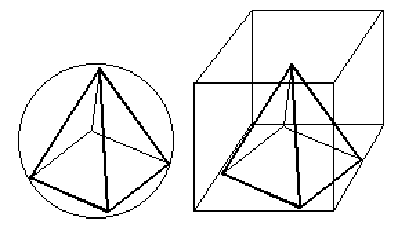
\includegraphics[width=0.6\textwidth]{img/shell.png}
		\caption{Сферическая и прямоугольная оболочки}
		\label{ref:img}}
\end{figure}

В дальнейшем при рассмотрении пересечения луча и объемной оболочкой
рассматриваемого объекта, если такого пересечения нет, то и соответственно пере­сечения
луча и самого рассматриваемого объекта нет, и наоборот, если будет найдено
пересечение, то возможно, есть пересечение луча и рассматриваемого объекта. Для
расчета эффектов освещения сцены проводятся вторичные лучи от точек пересече­ния
ко всем источникам света. Если на пути этих лучей встречается непрозрачное
тело, значит данная точка находится в тени, иначе он влияет на освещение данной
точки. Также для получения более реалистичного изображения сцены, нужно учи­тывать
вклады отраженных и преломленных лучей.
К недостатку алгоритма относится его производительность.

\section{Применение алгоритма}

Алгоритм трассировки лучей используется для визуализации
реалистического изображения, учитывая тени, отражение объектов, преломление и т.д.
Данный алгоритм активно используется, к примеру, в игровой индустрии.

\section{Параллельная реализация алгоритма обратной трассировки лучей}

Поскольку алгоритм обратной трассировки лучей обрабатывает каждый пиксель
экрана независимо, можно распараллелить обработку всего экрана, разбив
его на некоторые части. В данной лабораторной работе будет представлено 
разбиение горизонтально и вертикально. Т.е. каждый поток будет обрабатывать
свой участок экрана. 

На рис. \ref{ref:img1} показано, как можно вертикально разбить экран на 
несколько частей. На рис. \ref{ref:img2} показано горизонтальное разбиение экрана.
Разбив экран на части можно реализовывать параллельное вычисление цвета 
пикселей каждой части экрана.

\begin{figure}[ht!]
	\centering{
		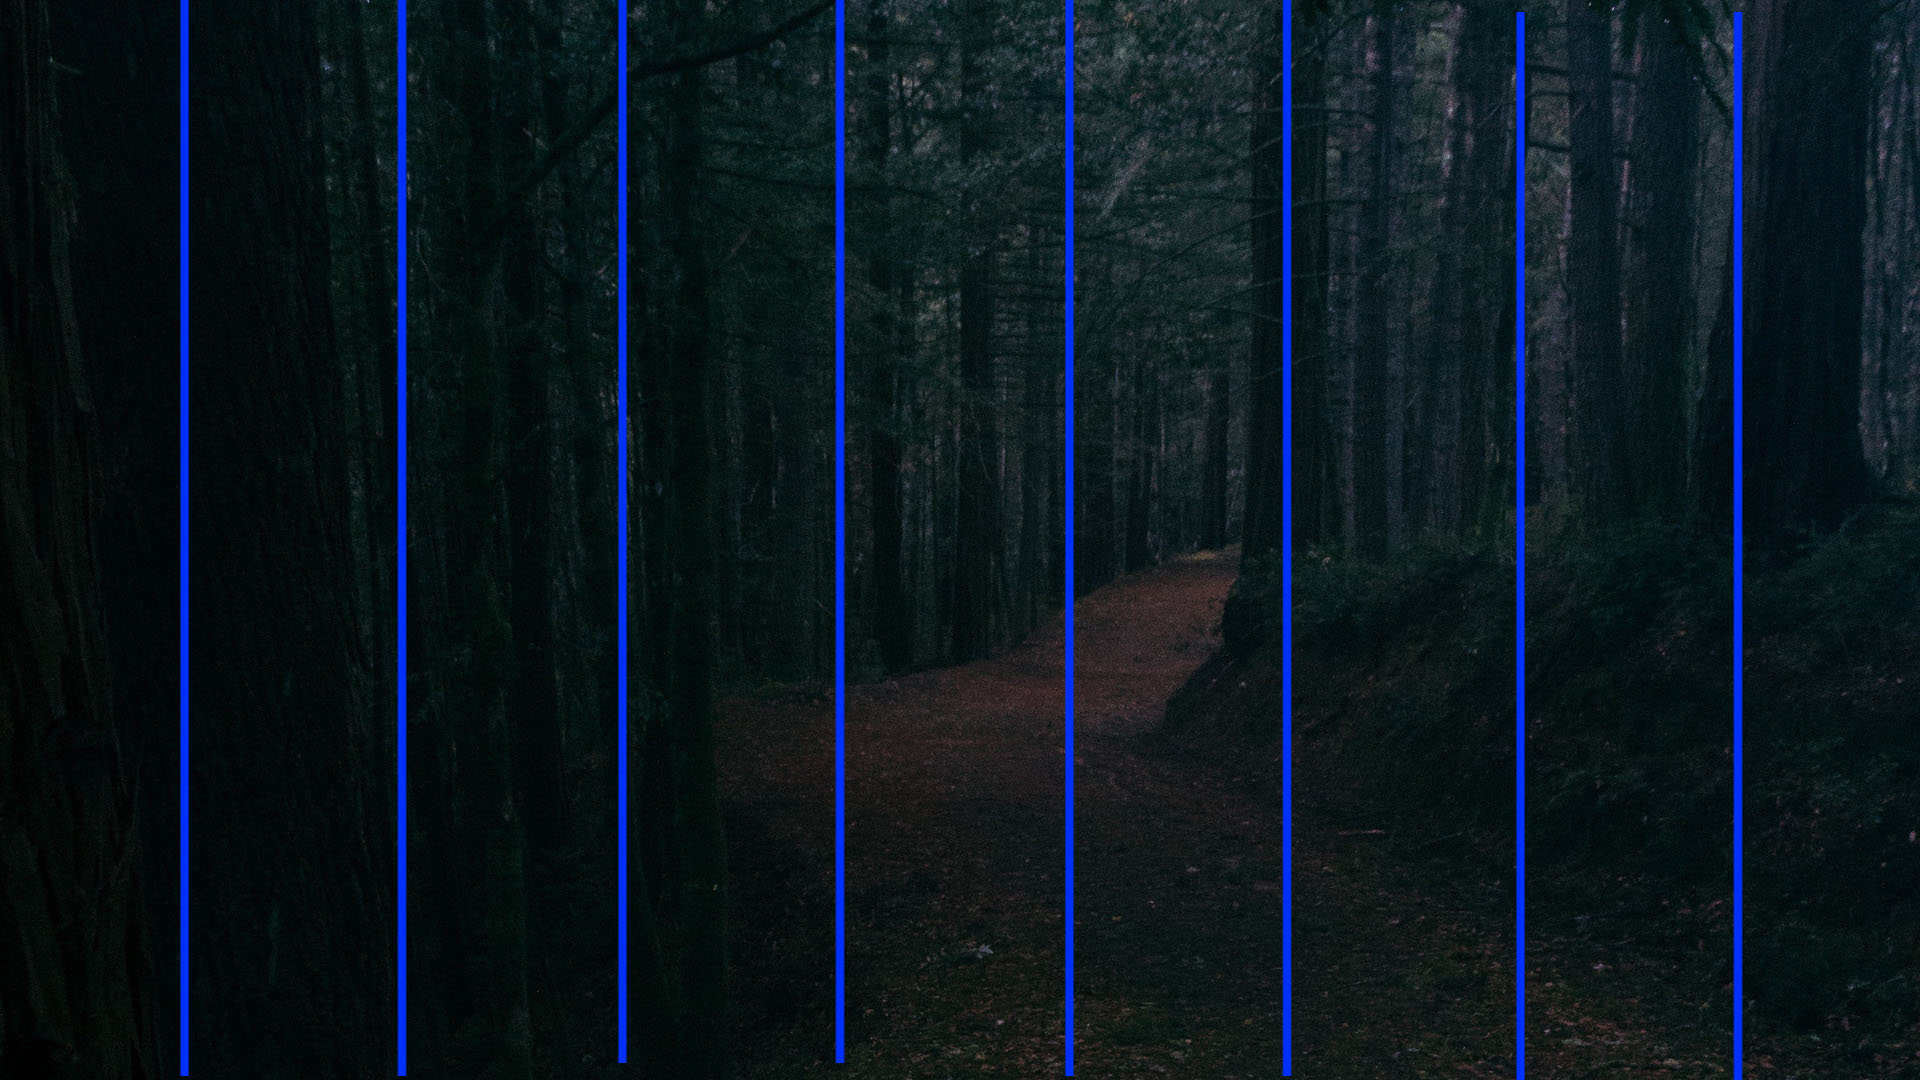
\includegraphics[width=0.8\textwidth]{img/h.jpg}
		\caption{Вертикальное разбиение экрана}
		\label{ref:img1}}
\end{figure}

\begin{figure}[ht!]
	\centering{
		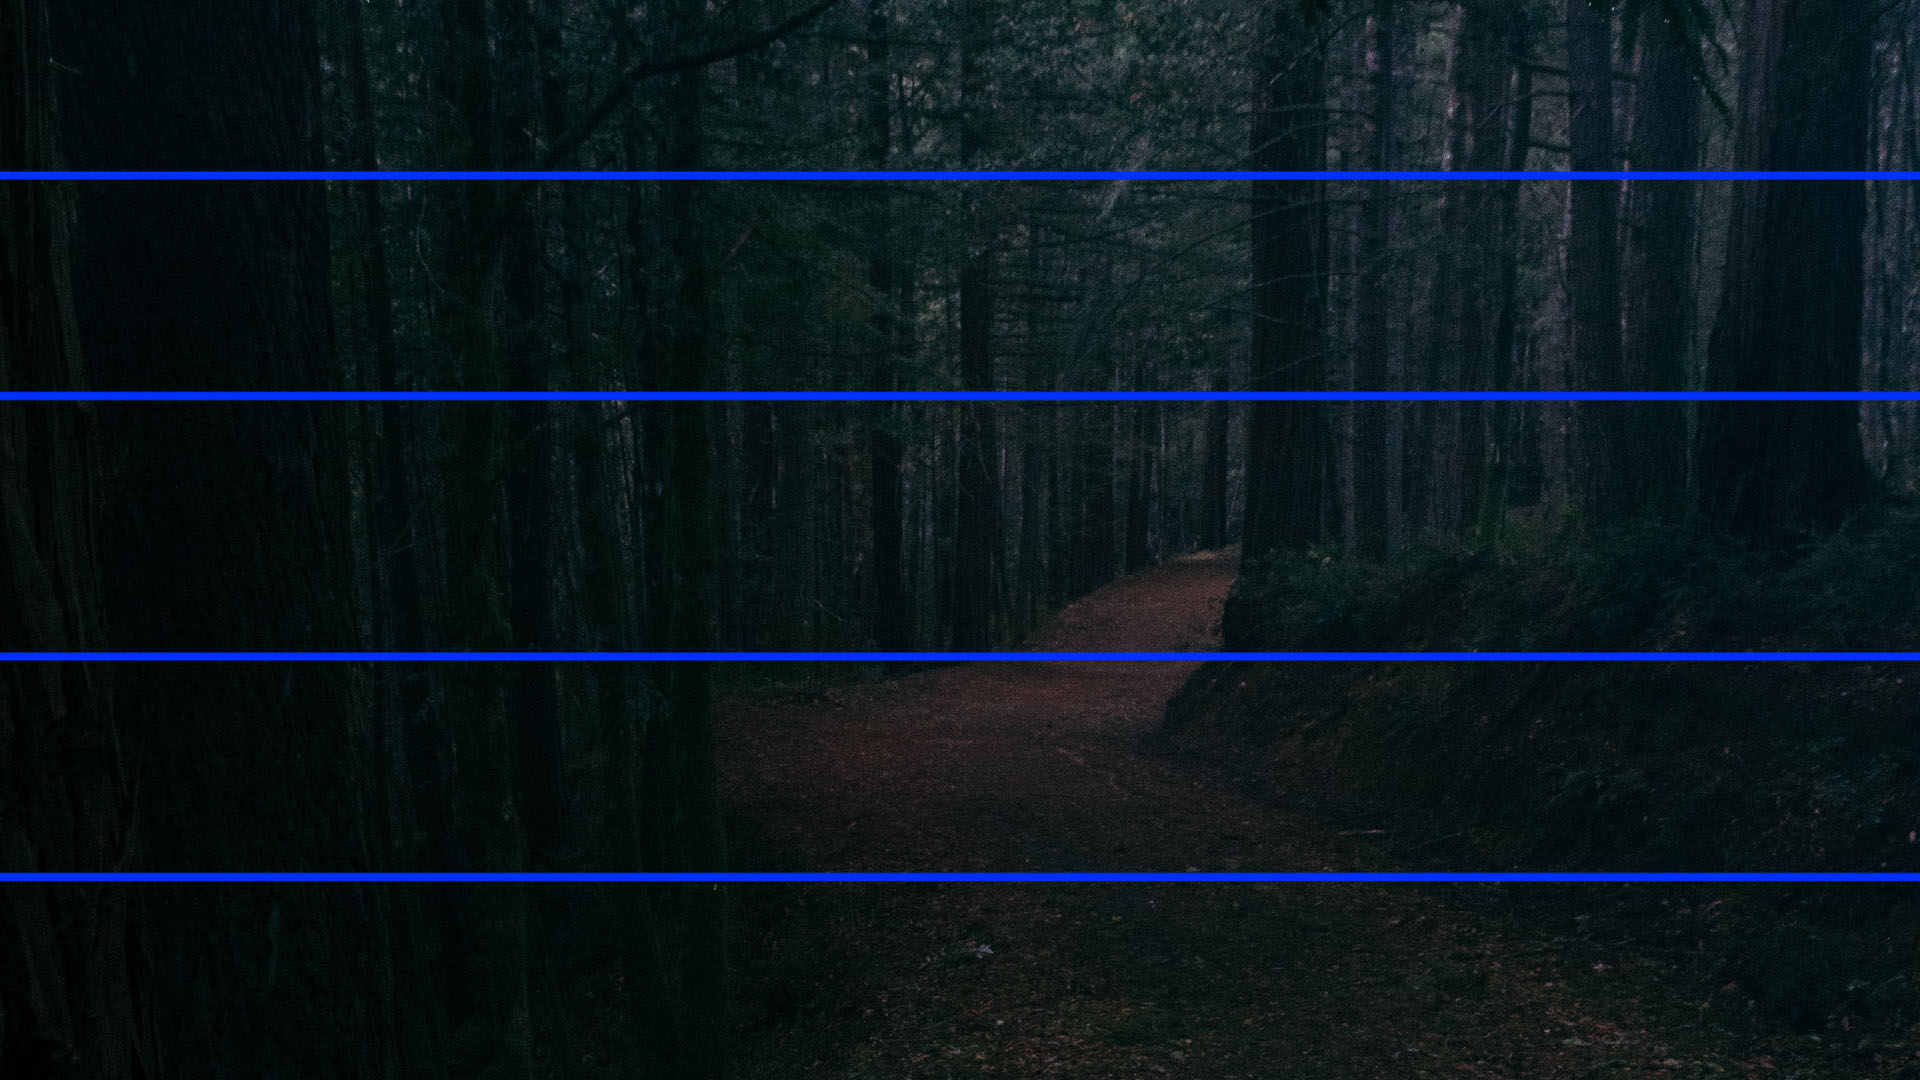
\includegraphics[width=0.8\textwidth]{img/w.jpg}
		\caption{Горизонтальное разбиение экрана}
		\label{ref:img2}}
\end{figure}

\section{Вывод}

В данном разделе были рассмотрены
основополагающие материалы, которые в дальнейшем потребуются
при параллельной и однопоточной реализации алгоритма трассировки лучей.  

\chapter{Конструкторский раздел}
\label{cha:design}
В данном разделе будут рассмотрены схемы алгоритмов умножения матриц.
На рис. \ref{fg:ref1} представлена схема стандартного алгоритма умножения матриц.

\begin{figure}[ht!]
	\centering{
		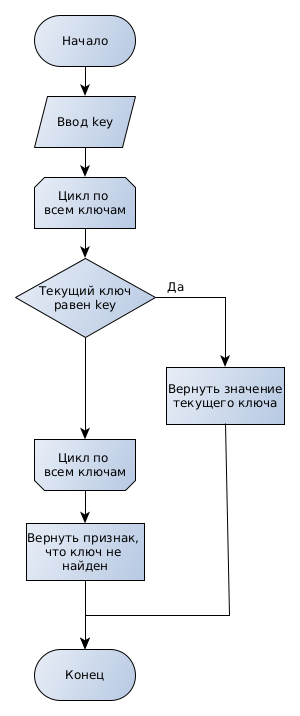
\includegraphics[width=0.6\textwidth]{img/d1.png}
		\caption{Схема стандартного алгоритма умножения матриц}
		\label{fg:ref1}}
\end{figure}



\section{Вывод}

В данном разделе были рассмотрены схемы (рис. \ref{fg:ref1} - \ref{fg:ref1}) алгоритмов умножения матриц.
\chapter{ Технологический раздел}
\label{cha:design}

\section{Выбор ЯП}

В данной лабораторной работе использовался язык программирования - python \cite{bib1}.
Данный язык простой и понятный, также я знакома с ним.
Поэтому данный язык был выбран. 
В качестве среды разработки я использовала Visual Studio Code \cite{bib2}, т.к. считаю его достаточно удобным и легким.
Visual Studio Code подходит не только для  Windows \cite{bib3}, но и для Linux \cite{bib4}, это еще одна причина, по которой я выбрала VS code, т.к. у меня установлена ОС Ubuntu 18.04.4 \cite{bib5}.

\section{Требования к программному обеспечению}

Входными данными являются две матрицы A и B.
Количество столбцов матрицы A долджно быть равно количеству строк матрицы B. 

На выходе получается результат умножения, введенных пользователем, матриц.

\section{Сведения о модулях программы}

Данная программа разбита на модули.

\begin{itemize}
    \item main.py - файл, содержащий точку входа в программу. В нем происходит общение с пользователем и вызов алгоритмов.
    \item matrix.py - файл, содержащий класс matrix.
    \item matrix\_multiplication.py - файл, содержащий реализации алгоритмов умножения матриц.
\end{itemize}

На листингах 3.1-3.4 представлен код программы.

\begin{lstlisting}[label=some-code,caption=Главная функция main]
def main():
    output("МАТРИЦА A", BLUE)
    n = int(input(GREEN + "Введите кол-во строк: "))
    m = int(input(GREEN + "Введите кол-во столбцов: "))
    output("Введите матрицу:", GREEN)
    matrixA = Matrix(n, m, [[int(j) for j in input(GREEN).split()]
                            for i in range(n)])

    output("МАТРИЦА B", BLUE)
    k = int(input(GREEN + "Введите кол-во строк: "))
    l = int(input(GREEN + "Введите кол-во столбцов: "))
    output("Введите матрицу:", GREEN)
    matrixB = Matrix(k, l, [[int(j) for j in input(GREEN).split()]
                            for i in range(k)])

    if m != k:
        output("Некорректные размеры матриц!", RED)
        return

    matrixC = multiplication(matrixA, matrixB)
    matrixC.output()
\end{lstlisting}

\begin{lstlisting}[label=some-code,caption=Класс matrix]
class Matrix:
    n, m = 0, 0
    matrix = list()

    def __init__(self, n, m, list_of_lists=None):
        self.n, self.m = n, m
        if list_of_lists:
            self.matrix = deepcopy(list_of_lists)
        else:
            self.matrix = np.full((n, m), 0)

    def output(self):
        print(TURQUOISE, end='')
        for i in range(self.n):
            for j in range(self.m):
                print(self.matrix[i][j], end=' ')
            print()

    def fill(self, list_of_lists):
        self.matrix = deepcopy(list_of_lists)

    def size(self):
        return (self.n, self.m)

    def __getitem__(self, index):
        return self.matrix[index]
\end{lstlisting}

\begin{lstlisting}[label=some-code,caption=Стандарный алгоритм умножения матриц]
    def multiplication(matrixA, matrixB):
        n = matrixA.n
        m = matrixB.m
        q = matrixB.n

        matrixC = Matrix(n, m)

        for i in range(n):
            for j in range(m):
                for k in range(q):
                    matrixC[i][j] += (matrixA[i][k] * matrixB[k][j])

        return matrixC
\end{lstlisting}

\begin{lstlisting}[label=some-code,caption=Алгоритм Винограда]
    def WinogradMult(matrixA, matrixB):
        n = matrixA.n
        m = matrixB.m
        q = matrixB.n

        matrixC = Matrix(n, m)

        tempA = np.full(n, 0)
        for i in range(n):
            for j in range(1, q, 2):
                tempA[i] += matrixA[i][j - 1] * matrixA[i][j]

        tempB = np.full(m, 0)
        for i in range(m):
            for j in range(1, q, 2):
                tempB[i] += matrixB[j - 1][i] * matrixB[j][i]

        for i in range(n):
            for j in range(m):
                matrixC[i][j] -= (tempA[i] + tempB[j])
                for k in range(1, q, 2):
                    matrixC[i][j] += (matrixA[i][k-1] + matrixB[k][j]) * \
                        (matrixA[i][k] + matrixB[k-1][j])
        if q % 2:
            for i in range(n):
                for j in range(m):
                    matrixC[i][j] += matrixA[i][q-1] * matrixB[q-1][j]

        return matrixC
\end{lstlisting}

\section{Тестирование}

В данном разделе будет приведена таблица с тестами (таблица \ref{table:ref1}).
% \ref{table:ref1}, в которой четко отражено тестирование программы

\begin{table}[ht]
    \centering
    \caption{Таблица тестов}
    \label{table:ref1}
    \begin{tabular}{ | l | l | l |}
        \hline
        Матрица A       & Матрица B           & Результат                               \\ \hline
        2 2 1 0 0 1     & 2 2 1 0 0 1         & Ответ верный                            \\ \hline
        3 2 2 3 1 0 2 2 & 2 4 2 2 1 9 4 2 8 1 & Ответ верный                            \\ \hline
        2 1 2 1         & 12 12               & Ответ верный                            \\ \hline
        2 2 1 0 0 1     & 1 1 0               & Сообщение о неверном вводе размерностей \\ \hline
        0 0             & 0 0                 &                                         \\ \hline
        \hline
    \end{tabular}
\end{table}

Все тесты пройдены.

\section{Вывод}

В данном разделе был разобран выбор языка программирования, а также среды разработки.
Разобраны требования к программному обеспечению.
Протестированная программа. 

\chapter{Экспериментальная часть}

В данном разделе сравним работу каждого алгоритма.

\section{Временные характеристики}

Сравним матричный алгоритм Левенштейна и Дамерау-Левенштейна.
Для сравнения возьмем строки длиной [10, 20, 30, 50, 100, 200]. 
Так как подсчет расстояния считается короткой задачей, мы воспользуемся усреднением массового эксперимента. 
Для этого сложим результат работы алгоритма n раз (n >= 10), после чего поделим на n. 
Тем самым мы получим достаточно точные характеристики времени. 
Сравнение произведем при n = 500.
Результат можно увидеть на рис.  \ref{fg:ref4}. Как мы можем наблюдать при короткой длине разница по времени минимальна, при увеличении длины строки алгоритм Левенштейна с небольшим опережением вырывается вперед. Это обосновывается тем, что у алгоритма Дамерау-Левенштейна задействуется еще одна операция, которая замедляет алгоритм.

\begin{figure}[ht!]
	\centering{
		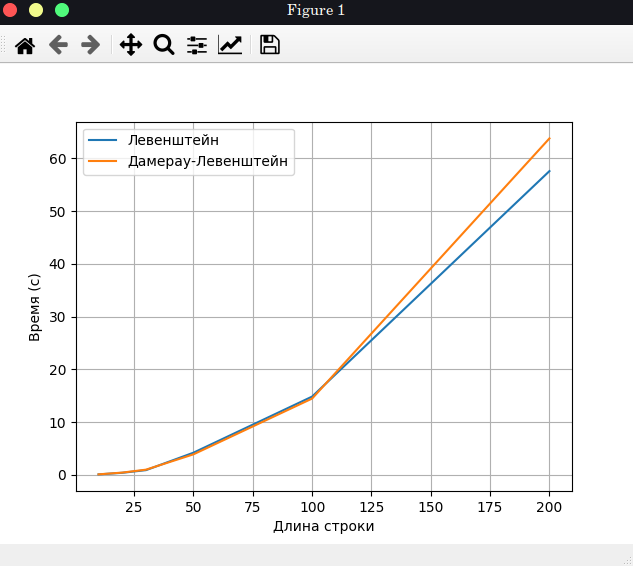
\includegraphics[width=0.6\textwidth]{img/graphLev-LevDam.png}
		\caption{Сравнение времени работы алгоритма Левенштейна и Дамерау-Левенштейна} 
		\label{fg:ref4}}
\end{figure}

Далее проведем сравнительный анализ временных характеристик рекурсивной и матричной реализаций алгоритма Левенштейна. 
Возьмем строки длиной [2, 3, 5, 7, 8], n положим равным 50.
Результат можно увидеть на рис. \ref{fg:ref5}.
Такая большая разница во времени объясняется тем, что в рекурсивном алгоритме Левенштейна много рекурсивных вызовов с однотипными параметрами.

\begin{figure}[ht!]
	\centering{
		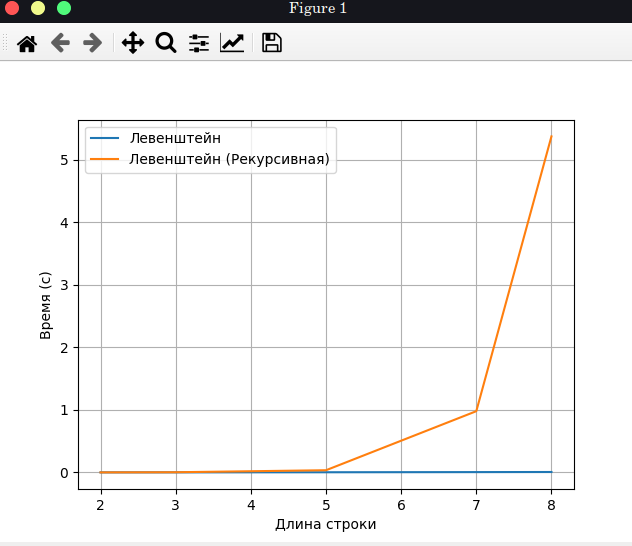
\includegraphics[width=0.6\textwidth]{img/graphLev-LevRec.png}
		\caption{Сравнение времени работы рекурсивной и матричной реализаций алгоритма Левенштейна.} 
		\label{fg:ref5}}
\end{figure}

\section{Характеристики по памяти}

На рисунке \ref{fg:ref6} представлено дерево вызовов рекурсивного алгоритма Левенштейна.
Видно, что на третьем уровне встречаются повторные вызовы. 
Чем больше будет уровень, тем чаще будут вызываться функции с однотипными аргументами, что может привести к превышению максимальной глубины рекурсии. 
При строках длиной 2 подпрограмма вызовется 18 раз. 
Каждый вызов задействует 32 мегабайт (замеры проведены с помощью  библиотеки memory\_profiler \cite{bib6}).
В итоге нам потребуется 576 мегабайт для рекурсивных вызовов, в то время, когда в матричном алгоритме используется 42 мегабайта. 

\begin{figure}[ht!]
	\centering{
		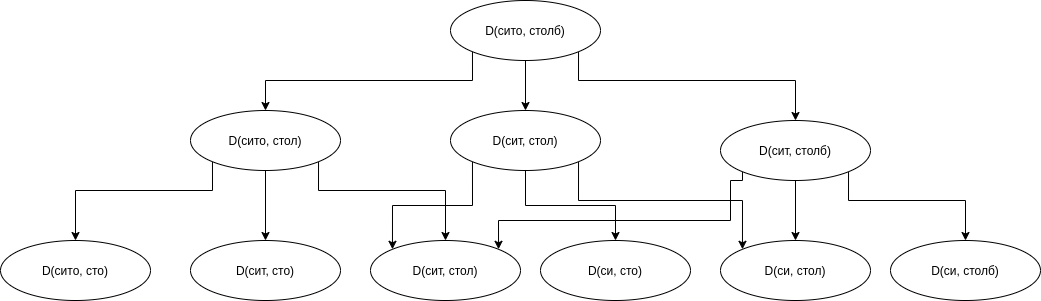
\includegraphics[width=0.8\textwidth]{img/rec_example.png}
		\caption{Сравнение времени работы рекурсивной и матричной реализаций алгоритма Левенштейна.} 
		\label{fg:ref6}}
\end{figure}

\section{Сравнительный анализ алгоритмов}

Приведенные характеристики показывают нам, что рекурсивная реализация алгоритма очень сильно проигрывает по времени и по памяти.\\
Во время печати очень часто возникают ошибки связанные с транспозицией букв, поэтому алгоритм Дамерау-Левенштейна предпочтительнее, не смотря на то, что он проигрывает по времени алгоритму Левенштейна.\\
По аналогии с первым абзацем можно сделать вывод о том, что рекуррентный алгоритм Дамерау-Левенштейна будет более затратный, как по памяти, так и по времени по сравнению с матричной реализацией Дамерау-Левенштейна.

\section{Вывод}

В данном разделе мы сравнили количество затраченного времени и памяти вышеизложенных алгоритмов. Самым быстрым оказался матричный алгоритм нахождения расстояния Левенштейна.





\backmatter %% Здесь заканчивается нумерованная часть документа и начинаются ссылки и
%% заключение

\chapter*{Заключение}
\addcontentsline{toc}{chapter}{Заключение}

В данной лабораторной работе были рассмотрены
основополагающие материалы которые в дальнейшем потребовались
при реализации конвейера.
Были рассмотрены схемы (рис. \ref{ref:d0} - \ref{ref:d1}) показывающие алгоритм конвейера.
Также были разобраны листинги рис 3.1-3.2,
показывающие работу контейнера и был приведен рис. \ref{ref:res},
показывающий корректную работу конвейера.
Был произведен сравнительный анализ рис. \ref{ref:time}.

В рамках выполнения работы решены следующие задачи:

\begin{enumerate}
	\item изучили освоили конвейерную обработку данных;
	\item применили изученные основы для реализации конвейерной обработки данных;
	\item получили практические навыки;
	\item получили статистику выполнения программы;
	\item описали и обосновали полученные результаты;
	\item выбрали и обосновали языка программирования, для решения данной задачи.
\end{enumerate}


% % Список литературы при помощи BibTeX
% Юзать так:
%
% pdflatex report
% bibtex report
% pdflatex report

\bibliographystyle{gost780u}
\bibliography{report}





%\appendix   % Тут идут приложения

\end{document}